\section{eo\-VRPInit Class Reference}
\label{classeo_v_r_p_init}\index{eoVRPInit@{eoVRPInit}}
Class defining the initializer functor.  


{\tt \#include $<$eo\-VRPInit.h$>$}

Inheritance diagram for eo\-VRPInit::\begin{figure}[H]
\begin{center}
\leavevmode
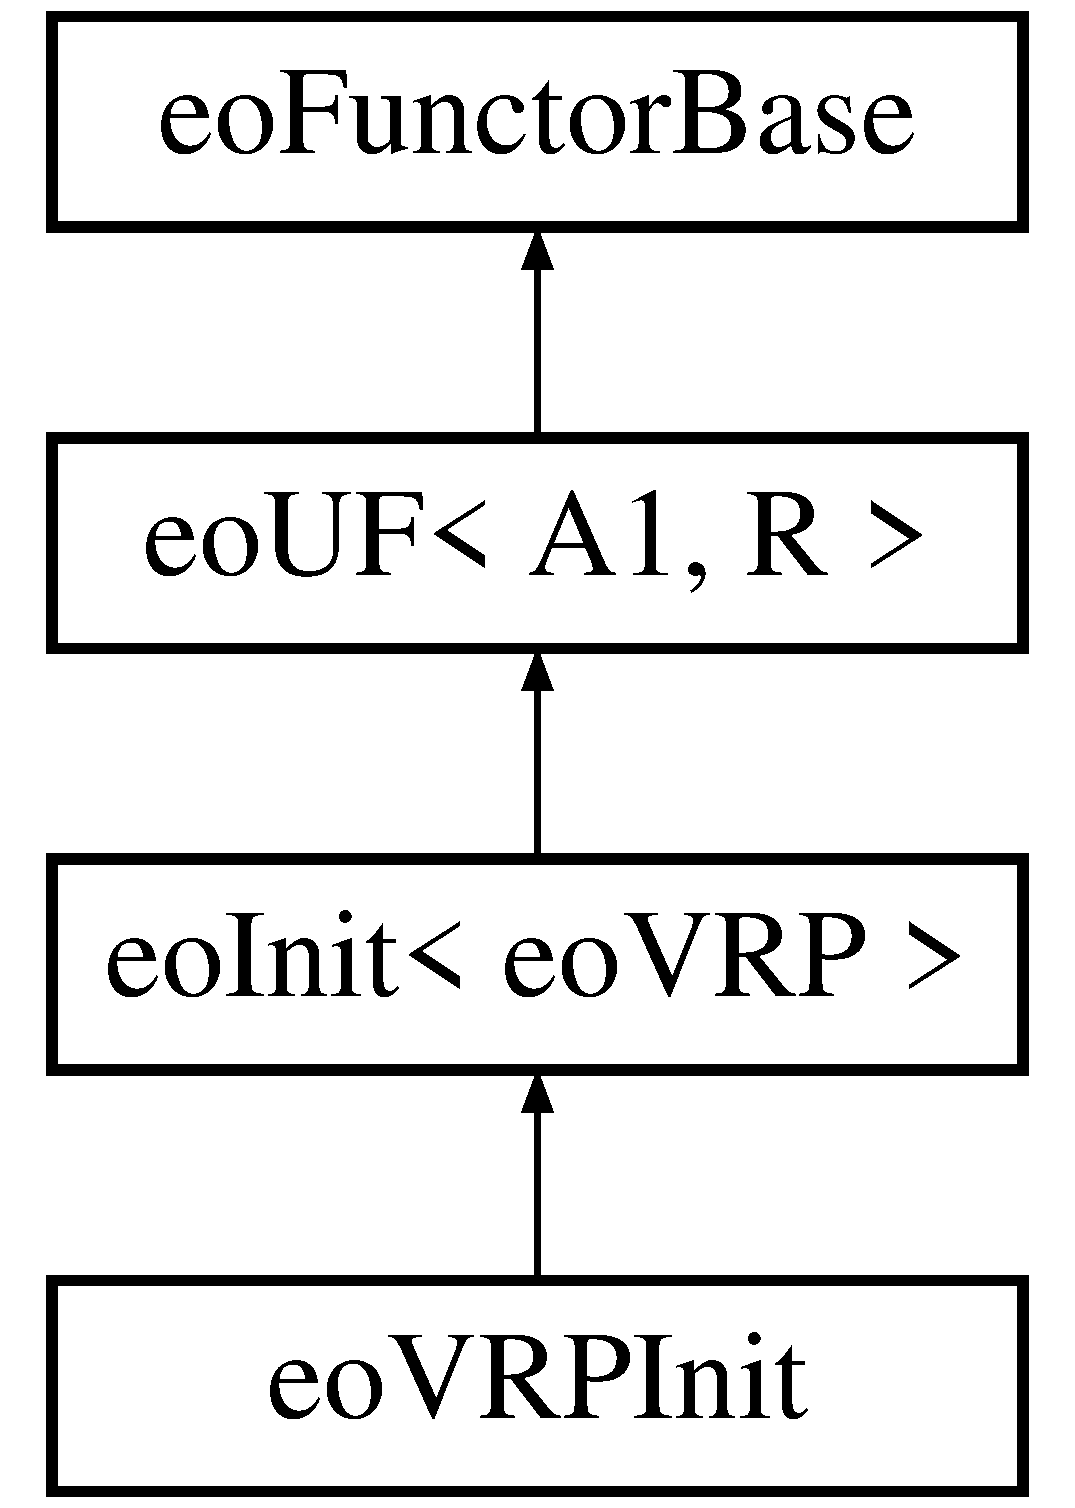
\includegraphics[height=4cm]{classeo_v_r_p_init}
\end{center}
\end{figure}
\subsection*{Public Member Functions}
\begin{CompactItemize}
\item 
\bf{eo\-VRPInit} ()\label{classeo_v_r_p_init_a620d4fa1b930b1fd8b491f1ef5c72fd}

\begin{CompactList}\small\item\em Default constructor: nothing to do here. \item\end{CompactList}\item 
void \bf{operator()} (\bf{eo\-VRP} \&\_\-gen)
\begin{CompactList}\small\item\em Functor member. \item\end{CompactList}\end{CompactItemize}
\subsection*{Private Member Functions}
\begin{CompactItemize}
\item 
void \bf{Heuristic\-Initialization} (\bf{eo\-VRP} \&\_\-gen)
\begin{CompactList}\small\item\em Heuristic initializer. \item\end{CompactList}\item 
bool \bf{create\-New\-Route} (std::vector$<$ int $>$ \&\_\-unvisited, int \&\_\-unvisited\-Idx, bool \_\-seed\-Checking\-Override, Route \&\_\-route)
\begin{CompactList}\small\item\em Creates a new route. \item\end{CompactList}\item 
bool \bf{select\-Best\-Insertion} (std::vector$<$ int $>$ \&\_\-unvisited, unsigned \_\-unvisited\-Idx, Route \&\_\-route, unsigned \&\_\-next\-Client, Route::iterator \&\_\-it)
\begin{CompactList}\small\item\em Selects the best client and the best position for its insertion in a given route. \item\end{CompactList}\item 
bool \bf{evaluate\-Insertion} (Route \&\_\-route, unsigned \_\-new\-Client, int \_\-after\-Client, double \&\_\-cost)
\begin{CompactList}\small\item\em Evaluates the feasibility and the cost of inserting a new client in a given subroute. \item\end{CompactList}\item 
unsigned \bf{select\-Farthest\-Client\-As\-Seed} (const std::vector$<$ int $>$ \&\_\-unvisited, int \_\-unvisited\-Idx)
\begin{CompactList}\small\item\em Selects the farthest client as seed for a new route. \item\end{CompactList}\item 
unsigned \bf{select\-Cheapest\-Client} (const std::vector$<$ int $>$ \&\_\-unvisited, int \_\-unvisited\-Idx, bool \_\-seed\-Checking\-Override)
\begin{CompactList}\small\item\em Selects the cheapest client as seed for a new route. \item\end{CompactList}\item 
unsigned \bf{select\-Best\-Client\-As\-Seed} (const std::vector$<$ int $>$ \&\_\-unvisited, int \_\-unvisited\-Idx, bool \_\-seed\-Checking\-Override)
\begin{CompactList}\small\item\em Selects the best (the \char`\"{}hardest\char`\"{} one) client as seed for a new route. \item\end{CompactList}\item 
void \bf{Random\-Initialization\-No\-Check} (\bf{eo\-VRP} \&\_\-gen)
\begin{CompactList}\small\item\em Random initializer. \item\end{CompactList}\end{CompactItemize}
\subsection*{Private Attributes}
\begin{CompactItemize}
\item 
unsigned \bf{m\-Seeds\-Used\-Count}\label{classeo_v_r_p_init_b74e164ca817fe5615e9519ec671a356}

\begin{CompactList}\small\item\em Number of clients already used as seeds. \item\end{CompactList}\item 
std::vector$<$ bool $>$ \bf{m\-Seeds\-Used}\label{classeo_v_r_p_init_5e940cc7eec88f268e8eb72313212947}

\begin{CompactList}\small\item\em Vector storing if a client has been used as a seed or not. \item\end{CompactList}\end{CompactItemize}


\subsection{Detailed Description}
Class defining the initializer functor. 

This class initializes an individual of the VRP problem using an heuristic initializer. 



Definition at line 65 of file eo\-VRPInit.h.

\subsection{Member Function Documentation}
\index{eoVRPInit@{eo\-VRPInit}!operator()@{operator()}}
\index{operator()@{operator()}!eoVRPInit@{eo\-VRPInit}}
\subsubsection{\setlength{\rightskip}{0pt plus 5cm}void eo\-VRPInit::operator() (\bf{eo\-VRP} \& {\em \_\-gen})\hspace{0.3cm}{\tt  [inline]}}\label{classeo_v_r_p_init_8bc4f6fb201b09dd882d721d2cfef8ce}


Functor member. 

Initializes a genotype using an heuristic initializer. \begin{Desc}
\item[Parameters:]
\begin{description}
\item[{\em \_\-gen}]Generally a genotype that has been default-constructed. Whatever it contains will be lost. \end{description}
\end{Desc}


Definition at line 99 of file eo\-VRPInit.h.

References Heuristic\-Initialization().\index{eoVRPInit@{eo\-VRPInit}!HeuristicInitialization@{HeuristicInitialization}}
\index{HeuristicInitialization@{HeuristicInitialization}!eoVRPInit@{eo\-VRPInit}}
\subsubsection{\setlength{\rightskip}{0pt plus 5cm}void eo\-VRPInit::Heuristic\-Initialization (\bf{eo\-VRP} \& {\em \_\-gen})\hspace{0.3cm}{\tt  [inline, private]}}\label{classeo_v_r_p_init_af5946da88fb14494cb23dc21d167866}


Heuristic initializer. 

This initializer constructs and individual from routes. Each route is built in a constructive way. The first client of each route is selected trying to maximize a function depending on its time window and how far it is from the depot. We always try to select the hardest clients as seeds. Used seeds are stored so that different seeds are selected for different individuals and thus guarantee the diversity of the initial population. \begin{Desc}
\item[Parameters:]
\begin{description}
\item[{\em \_\-gen}]The individual to be initialized. \end{description}
\end{Desc}


Definition at line 123 of file eo\-VRPInit.h.

References eo\-VRPUtils::clients, create\-New\-Route(), and EO$<$ F $>$::invalidate().

Referenced by operator()().\index{eoVRPInit@{eo\-VRPInit}!createNewRoute@{createNewRoute}}
\index{createNewRoute@{createNewRoute}!eoVRPInit@{eo\-VRPInit}}
\subsubsection{\setlength{\rightskip}{0pt plus 5cm}bool eo\-VRPInit::create\-New\-Route (std::vector$<$ int $>$ \& {\em \_\-unvisited}, int \& {\em \_\-unvisited\-Idx}, bool {\em \_\-seed\-Checking\-Override}, Route \& {\em \_\-route})\hspace{0.3cm}{\tt  [inline, private]}}\label{classeo_v_r_p_init_ff7c0bf38bdd70d6f9d561479ec4f48a}


Creates a new route. 

Creates a new route selecting the best (hardest) client as seed and then adding the cheapest clients until one of the constraints (time window or vehicle's capacity) is broken. \begin{Desc}
\item[Parameters:]
\begin{description}
\item[{\em \_\-unvisited}]Vector of unvisited and thus available clients for constructing the new route. \item[{\em \_\-unvisited\-Idx}]Position of the last univisted client in \_\-unvisited vector. \item[{\em \_\-seed\-Checking\-Override}]If true, it overrides the seed checking mecanism. It must be always false for the first route and then true for the following ones. This way we will preserve diversity in our initial population as every individual will be initialized from a different initial route. \item[{\em \_\-route}]The brand new route we have constructed. \end{description}
\end{Desc}
\begin{Desc}
\item[Returns:]True if everything went ok. \end{Desc}


Definition at line 176 of file eo\-VRPInit.h.

References m\-Seeds\-Used, m\-Seeds\-Used\-Count, select\-Best\-Client\-As\-Seed(), and select\-Best\-Insertion().

Referenced by Heuristic\-Initialization().\index{eoVRPInit@{eo\-VRPInit}!selectBestInsertion@{selectBestInsertion}}
\index{selectBestInsertion@{selectBestInsertion}!eoVRPInit@{eo\-VRPInit}}
\subsubsection{\setlength{\rightskip}{0pt plus 5cm}bool eo\-VRPInit::select\-Best\-Insertion (std::vector$<$ int $>$ \& {\em \_\-unvisited}, unsigned {\em \_\-unvisited\-Idx}, Route \& {\em \_\-route}, unsigned \& {\em \_\-next\-Client}, Route::iterator \& {\em \_\-it})\hspace{0.3cm}{\tt  [inline, private]}}\label{classeo_v_r_p_init_7f07be1f3a027dc56af84bb46828ddda}


Selects the best client and the best position for its insertion in a given route. 

Given a subroute, this method tries to find the best client and the best position for it among all the univisited clients. \begin{Desc}
\item[Parameters:]
\begin{description}
\item[{\em \_\-unvisited}]Vector of unvisited and thus available clients for constructing the new route. \item[{\em \_\-unvisited\-Idx}]Position of the last univisted client in \_\-unvisited vector. \item[{\em \_\-route}]The route where we are trying to insert a new client. \item[{\em \_\-next\-Client}]A return value. The selected client to be inserted. \item[{\em \_\-it}]A return value. The position for selected client to be inserted. \end{description}
\end{Desc}
\begin{Desc}
\item[Returns:]True if a new insertion is possible. False otherwise. \end{Desc}


Definition at line 249 of file eo\-VRPInit.h.

References evaluate\-Insertion().

Referenced by create\-New\-Route().\index{eoVRPInit@{eo\-VRPInit}!evaluateInsertion@{evaluateInsertion}}
\index{evaluateInsertion@{evaluateInsertion}!eoVRPInit@{eo\-VRPInit}}
\subsubsection{\setlength{\rightskip}{0pt plus 5cm}bool eo\-VRPInit::evaluate\-Insertion (Route \& {\em \_\-route}, unsigned {\em \_\-new\-Client}, int {\em \_\-after\-Client}, double \& {\em \_\-cost})\hspace{0.3cm}{\tt  [inline, private]}}\label{classeo_v_r_p_init_82f2bb762d8f5da85febd266fb75a29b}


Evaluates the feasibility and the cost of inserting a new client in a given subroute. 

Given a subroute, this method tries evaluates if it is possible to insert a client in a position. It will return the cost of the resulting route if this insertion is possible. \begin{Desc}
\item[Parameters:]
\begin{description}
\item[{\em \_\-route}]The route where we are trying to insert a new client. \item[{\em \_\-new\-Client}]The client we are trying to insert. \item[{\em \_\-after\-Client}]The position of insertion. \item[{\em \_\-cost}]A return value. The cost of inserting the given client at the given position. \end{description}
\end{Desc}
\begin{Desc}
\item[Returns:]True if the new insertion is possible. False otherwise. \end{Desc}


Definition at line 308 of file eo\-VRPInit.h.

References eo\-VRPUtils::clients, eo\-VRPUtils::distance(), and eo\-VRPUtils::get\-Time\-Window().

Referenced by select\-Best\-Insertion().\index{eoVRPInit@{eo\-VRPInit}!selectFarthestClientAsSeed@{selectFarthestClientAsSeed}}
\index{selectFarthestClientAsSeed@{selectFarthestClientAsSeed}!eoVRPInit@{eo\-VRPInit}}
\subsubsection{\setlength{\rightskip}{0pt plus 5cm}unsigned eo\-VRPInit::select\-Farthest\-Client\-As\-Seed (const std::vector$<$ int $>$ \& {\em \_\-unvisited}, int {\em \_\-unvisited\-Idx})\hspace{0.3cm}{\tt  [inline, private]}}\label{classeo_v_r_p_init_a24867d25a6c9911e9b5c9eb1b4b650d}


Selects the farthest client as seed for a new route. 

\begin{Desc}
\item[Parameters:]
\begin{description}
\item[{\em \_\-unvisited}]Vector of unvisited and thus available clients for constructing the new route. \item[{\em \_\-unvisited\-Idx}]Position of the last univisted client in \_\-unvisited vector. \end{description}
\end{Desc}
\begin{Desc}
\item[Returns:]The position of the client farthest from the depot. \end{Desc}


Definition at line 472 of file eo\-VRPInit.h.

References eo\-VRPUtils::distance().\index{eoVRPInit@{eo\-VRPInit}!selectCheapestClient@{selectCheapestClient}}
\index{selectCheapestClient@{selectCheapestClient}!eoVRPInit@{eo\-VRPInit}}
\subsubsection{\setlength{\rightskip}{0pt plus 5cm}unsigned eo\-VRPInit::select\-Cheapest\-Client (const std::vector$<$ int $>$ \& {\em \_\-unvisited}, int {\em \_\-unvisited\-Idx}, bool {\em \_\-seed\-Checking\-Override})\hspace{0.3cm}{\tt  [inline, private]}}\label{classeo_v_r_p_init_0bb48de33e92c2b6a386e28d5b759f4b}


Selects the cheapest client as seed for a new route. 

\begin{Desc}
\item[Parameters:]
\begin{description}
\item[{\em \_\-unvisited}]Vector of unvisited and thus available clients for constructing the new route. \item[{\em \_\-unvisited\-Idx}]Position of the last univisted client in \_\-unvisited vector. \item[{\em \_\-seed\-Checking\-Override}]If true, it overrides the seed checking mecanism. \end{description}
\end{Desc}
\begin{Desc}
\item[Returns:]The position of the cheapest client. \end{Desc}


Definition at line 498 of file eo\-VRPInit.h.

References eo\-VRPUtils::clients, eo\-VRPUtils::distance(), eo\-Rng::flip(), m\-Seeds\-Used, and eo\-VRPUtils::polar\-Angle().\index{eoVRPInit@{eo\-VRPInit}!selectBestClientAsSeed@{selectBestClientAsSeed}}
\index{selectBestClientAsSeed@{selectBestClientAsSeed}!eoVRPInit@{eo\-VRPInit}}
\subsubsection{\setlength{\rightskip}{0pt plus 5cm}unsigned eo\-VRPInit::select\-Best\-Client\-As\-Seed (const std::vector$<$ int $>$ \& {\em \_\-unvisited}, int {\em \_\-unvisited\-Idx}, bool {\em \_\-seed\-Checking\-Override})\hspace{0.3cm}{\tt  [inline, private]}}\label{classeo_v_r_p_init_dd681a23869f69438120ee2d82f85e94}


Selects the best (the \char`\"{}hardest\char`\"{} one) client as seed for a new route. 

\begin{Desc}
\item[Parameters:]
\begin{description}
\item[{\em \_\-unvisited}]Vector of unvisited and thus available clients for constructing the new route. \item[{\em \_\-unvisited\-Idx}]Position of the last univisted client in \_\-unvisited vector. \item[{\em \_\-seed\-Checking\-Override}]If true, it overrides the seed checking mecanism. \end{description}
\end{Desc}
\begin{Desc}
\item[Returns:]The position of the best client. \end{Desc}


Definition at line 532 of file eo\-VRPInit.h.

References eo\-VRPUtils::clients, eo\-VRPUtils::distance(), eo\-Rng::flip(), m\-Seeds\-Used, and eo\-Rng::uniform().

Referenced by create\-New\-Route().\index{eoVRPInit@{eo\-VRPInit}!RandomInitializationNoCheck@{RandomInitializationNoCheck}}
\index{RandomInitializationNoCheck@{RandomInitializationNoCheck}!eoVRPInit@{eo\-VRPInit}}
\subsubsection{\setlength{\rightskip}{0pt plus 5cm}void eo\-VRPInit::Random\-Initialization\-No\-Check (\bf{eo\-VRP} \& {\em \_\-gen})\hspace{0.3cm}{\tt  [inline, private]}}\label{classeo_v_r_p_init_008ae39692b67ef0b25aed89075b1d46}


Random initializer. 

Initializes a genotype using a random initializer. \begin{Desc}
\item[Parameters:]
\begin{description}
\item[{\em \_\-gen}]Generally a genotype that has been default-constructed. Whatever it contains will be lost. \end{description}
\end{Desc}


Definition at line 569 of file eo\-VRPInit.h.

References eo\-VRPUtils::clients, and eo\-Rng::random().

The documentation for this class was generated from the following file:\begin{CompactItemize}
\item 
eo\-VRPInit.h\end{CompactItemize}
